%!TEX root = ../thesis.tex
%*******************************************************************************
%*********************************** First Chapter *****************************
%*******************************************************************************

\chapter{Introduction}  %Title of the First Chapter

\ifpdf
    \graphicspath{{Chapter1/Figs/Raster/}{Chapter1/Figs/PDF/}{Chapter1/Figs/}}
\else
    \graphicspath{{Chapter1/Figs/Vector/}{Chapter1/Figs/}}
\fi

The advent of the Internet of Things (IoT) has brought the need for novel studies to conform to its extensive requirements, driven specifically by the Smart Vehicle industry.   Smart vehicles must be able to efficiently sense and communicate with other nearby vehicles, including cars, buses and trucks. For obvious reasons, the design and specification of microelectronic circuits, which are used in these applications, are regulated by many strict security and safety standards. Reliability and robustness in the device operation must be ensured for harsh environments \cite{Ferreira2014}, including the required operating temperature range from -40 $^{\circ}$C to 175 $^{\circ}$C. This temperature range is arguably the most difficult environment challenge for electronics in the automotive industry \cite{Chain1997}. Hence, to meet the IoT challenge, smart vehicles must integrate high performance electronics over a wide temperature range.

Such electronics are challenged by the high temperature near engine, disc brake systems and abrupt accelerations worsen the difficulty of smart actuator design. Information on automotive environments and electrical component test standards can be found at the Automotive Electronics Council~\cite{1393072,ISO16750}. \figurename~\ref{fig:automotive-cond} shows the typical temperature environment for such embedded electronics. The operating temperature is a function of the location, the circuit's power dissipation, and the thermal design. Noting that typical junction temperature for integrated circuits are 10\(\degree \)C to 25\(\degree \)C higher than ambient temperature, the on-engine temperature specification is often -40\(\degree \)C to 175\(\degree \)C.

\begin{figure}[htp]
	\centering
	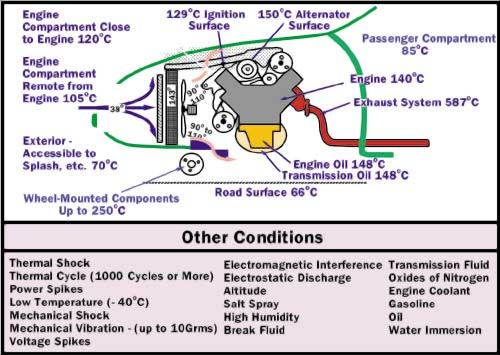
\includegraphics[width=.8\textwidth]{Chapter1/Figs/automotive_cond.png}
	\caption{Stringent automotive conditions presented by the Automotive Electronics Council~\cite{1393072,ISO16750}}
	\label{fig:automotive-cond}
\end{figure}

Aiming a Smart Vehicle, the sensor market is arguably the most important one. The vehicle smartness is given by strong processing unit which could not stand the harsh environment in which most of sensors should sustain. To transfer the information of sensors to those processing units, it is mandatory to place the Analog-to-Digital converters (ADC) as closer as possible to the sensor with a sampling rate sufficiently high for the future application of autonomous car. For all these reasons, ADC design is a challenge since it should remain reliable even under performance variation \cite{Cai2012}.

%********************************** %First Section  **************************************
\section{Motivation}   % section 1.1
To that extent, a low-cost, fast and accurate ADC operating in those harsh conditions is a good ally for equipment manufacturers. To decrease the cost, the area is a major concern. Considering re-use of the ADC as an IP-bloc, the area has been limited to less than half a square millimeter.
In the automotive environment, ADCs are the usual interface with environmental sensors and motor control sensors. 

\begin{table}[htp]
	\centering
	\caption{Specification of target ADC}
	\label{tbl:adc-spec}
	\rowcolors{2}{gray!15}{white}
	\begin{tabular}{ll}
		\toprule
		& Criterion                                                                                                                                                   \\ \midrule
		Operating Temperature            & -40 $\degree$ C -- +175 $\degree$ C                                                                                               \\
		Supply Voltage                   & 1.8 V $\pm$ 10 \%                                                                                                                              \\
		Differential Input Voltage Range & $\pm$ 1V                                                                                                                                       \\
		Area                             & \textless 0.5 \(mm^2\)                                                                                                                                      \\
		Conversion Speed                 & 20 MSamples/s                                                                                                                                               \\
		Maximum Clock Frequency          & 100 MHz\\
		Clock Duty-Cycle                 & 40 -- 60 \%                                                                                                                                                 \\
		Latency                          & 500 ns                                                                                                                                                      \\
		Resolution                       & $\geq$ 12-bits                                                                                          \\
		\rowcolor{white}\multirow{-3}{*}{SNDR }   & min 74 dB for $F_s$ \textless 5 MHz\\
		\rowcolor{white}                      & min 68 dB for 5 MHz \textless $F_s$  \textless 10 MHz,\\
		\rowcolor{white}						& min 62 dB for $F_s$  \textgreater 10 MHz  \\
		SFDR (Full-Scale)                & min 68 dB                                                                                               \\
		DNL                              & \textless LSB/2                                                                                       \\
		INL                              & \textless LSB/2 best-fit method                                                                                    \\
		Offset Error                     & \textless 4 LSB                                                                                                                                             \\
		Gain Error                       & \textless 4 LSB                                                                                                                                             \\
		Adjacent ADC mismatch Error      & \textless 4 LSB                                                                                                                                             \\
		Energy, $E_s = P/F_s$            & 0.75 nJ/sample      \\ \bottomrule                                                                                                                                       
	\end{tabular}
\end{table}

\nomenclature[z]{PVT}{Process-Voltage-Temperature}
The frequency spectrum of such application being limited, the ADC does not need to tackle for Gigahertz sampling. The accuracy and the linearity is of much importance. Nevertheless, vehicle communicates the sensors information. To receive them, the bandwidth of the signal is few megahertz.
To fulfill the need, the minimum requirements for a final product are listed in Table~\ref{tbl:adc-spec}. The order of importance is the area, the resolution, the power consumption, and the conversion speed. It is important to highlight the temperature range and the ratio between the conversion speed and the maximum clock frequency equal to 5. This ratio also called Oversampling Ratio (OSR) is the number of clock cycle allowed to perform a conversion.

To responds to the future need of the automotive environment, we aim a design of an ADC over a wide temperature range from -40\(\degree \)C to 175\(\degree \)C with the following characteristics:

\begin{itemize}
	\item Maximum oversampling ratio of 5
	\item SNDR greater than 68 dB
	\item a consumption less than 0.75 nJ/sample
	\item and target a silicon area less than 0.5 \(mm^2 \) for cost reason
\end{itemize}
 
With a preference sets on the minimization of the silicon area, before the minimization of the power consumption, the resolution and the speed.

\section{Thesis Organisation}

This work focuses on the design of high-precision, high-speed and energy efficient ADC under the harsh environment the automotive one represents. A emphasis is on doing such design in a SOI CMOS processes under stringent Process-Voltage-Temperature (PVT) variations. Our main contribution relies on the development of a new hybrid topology proposal using 3 stages to cope with such constraints based on a top-down approach: a counting stage inherently linear, an algorithmic stage to increase rapidly the precision, and a SAR stage for area and power consumption trade-off.

We review operation of conventional ADC topologies in the Chapter~\ref{sec:soa}. Their advantages and source of errors are discussed to present why some architectures are predominant in high temperature conditions. Namely, few of them such as \(\Delta \Sigma\), SAR, and pipelined are able to cope with analog imperfections coming from the temperature. The proposed architecture is then presented to benefit from the strength of each one.

The section~\ref{sec:temperature-analogue} then discusses the challenge of analog design over a large temperature range from -40\(\degree\)C to +175\(\degree\)C. Phenomena tightly linked to the temperature are analysed to highlight the design trade-offs when considering temperature effects. Based on a \(g_m/I_D\) methodology, the insight gained from this analysis is then reused during the design phase.

Having the severe degradation, we discuss enhancement ported to our topology proposal to glean the maximum of performances within the smallest footprint in a 180 nm technology. Alongside the optimization, Chapter~\ref{sec:adc-implementation} considers the reliability and introduces the case of pseudo-asynchronous design to relax timing restrictions in the digital part over temperature. We have defined a methodology for the design and characterization of such converter by using a testbench comparing a high-level model of the converter, defined in VerilogAMS, and a schematic description of the converter, able to use macromodels of the components or their transistor-level description. A MATLAB post-processing can extract the main characteristics such as the precision, the INL, DNL ...

The design of mandatory analog blocks, which are respectively comparators and operational amplifier, is examined to ensure the expected behavior for a rigorous 6\(\sigma\) process variation. To achieve this, a new time delay model have been developed for the Double Tail latch. This model has been presented during the ECCTD conference held in 2017. Meanwhile, the layout concerns to get the most of the op-amp is also discussed in the Chapter~\ref{sec:analog-building-bloc}.

Despite the fact the ADC testchip is in a finalization stage, experimentation is key in the validation process of IP components. Details in the realization of testchips in temperature which are worth to be discussed are presented in Chapter~\ref{sec:tests-meas}. With a chip dedicated for the assessment of comparators, their offset, the delay, the noise, and the hysteresis measurement circuits are implemented. The delay of high speed clocked comparator has been measured with a new measurement circuits presented during the ECCTD in 2017. After the enhancement of our topology proposal, only the testability of the last stage has seen its complexity increased. A second test chip assesses the effectiveness of pseudo-asynchronous design at high temperature and extracts static metrics of the last stage (DNL, INL, ...). Then, a last section focuses on the ADC testchip. Its design and preliminary results of the ADC are presented. Chapter~\ref{sec:perspectives} concludes our research findings and suggests potential future work.
